\chapter{О мире CodeBall 2018}

\newcommand{\const}[1]{\texttt{#1}}

\section{Общие положения игры и правила проведения турнира}

Данное соревнование предоставляет вам возможность проверить свои навыки программирования,
создав искусственный интеллект (стратегию),
управляющий командой роботов в специальном игровом мире
(подробнее об особенностях мира CodeBall 2018 можно узнать в следующих пунктах этой главы).
В зависимости от этапа соревнования у вас в команде будет от 2 до 3 роботов,
а также может быть доступно либо недоступно использование нитро.
Все роботы одинаковы по параметрам и являются шарами, исходное расположение гарантированно симметричное.
Помимо самих роботов в игре также есть мяч.

В каждой игре вам будет противостоять стратегия другого игрока.
Цель вышей команды --- забрасывать мяч в ворота противника и мешать попаданию мяча в свои ворота.
Команда, забившая больше голов, объявляется победителем.
Игра может закончиться и ничьей, если обе команды забили одинаковое количество голов.

Турнир проводится в несколько этапов, которым предшествует квалификация в Песочнице.
Песочница --- соревнование, которое проходит на протяжении всего чемпионата.
В рамках каждого этапа игроку соответствует некоторое значение рейтинга ---
показателя того, насколько успешно его стратегия участвует в играх.

Начальное значение рейтинга в Песочнице равно $1200$.
По итогам игры это значение может как увеличиться, так и уменьшиться.
При этом победа над слабым (с низким рейтингом) противником даёт небольшой прирост,
также и поражение от сильного соперника незначительно уменьшает ваш рейтинг.
Со временем рейтинг в Песочнице становится всё более инертным,
что позволяет уменьшить влияние случайных длинных серий побед или поражений на место участника,
однако вместе с тем и затрудняет изменение его положения при существенном улучшении стратегии.
Для отмены данного эффекта участник может сбросить изменчивость рейтинга до начального состояния при отправке новой стратегии,
включив соответствующую опцию.
В случае принятия новой стратегии системой рейтинг участника сильно упадёт после следующей игры в Песочнице,
однако по мере дальнейшего участия в играх быстро восстановится и даже станет выше,
если ваша стратегия действительно стала эффективнее.
Не рекомендуется использовать данную опцию при незначительных, инкрементальных улучшениях вашей стратегии,
а также в случаях, когда новая стратегия недостаточно протестирована и эффект от изменений в ней достоверно не известен.

Начальное значение рейтинга на каждом основном этапе турнира равно $0$.
За каждую игру участник получает определённое количество единиц рейтинга в зависимости от занятого места
Если два или более участников делят какое-то место,
то суммарное количество единиц рейтинга за это место и за следующие
$\texttt{количество\_таких\_участников}-1$ мест делится поровну между этими участниками.
Например, если два участника делят первое место,
то каждый из них получит половину от суммы единиц рейтинга за первое и второе места.
При делении округление всегда совершается в меньшую сторону.
Более подробная информация об этапах турнира будет предоставлена в анонсах на сайте проекта.

Сначала все участники могут участвовать только в играх, проходящих в Песочнице.
Игроки могут отправлять в Песочницу свои стратегии,
и последняя принятая из них берётся системой для участия в квалификационных играх.
Каждый игрок участвует примерно в одной квалификационной игре за час.
Жюри оставляет за собой право изменить этот интервал, исходя из пропускной способности тестирующей системы,
однако для большинства участников он остаётся постоянной величиной.
Существует ряд критериев, по которым интервал участия в квалификационных играх может быть увеличен для конкретного игрока.
За каждую N-ю полную неделю, прошедшую с момента отправки игроком последней стратегии,
интервал участия для этого игрока увеличивается на N базовых интервалов тестирования.
Учитываются только принятые системой стратегии.
За каждое <<падение>> стратегии в $10$ последних играх в Песочнице начисляется дополнительный штраф,
равный $20\%$ от базового интервала тестирования.
Подробнее о причинах <<падения>> стратегии можно узнать в следующих разделах.
Интервал участия игрока в Песочнице не может стать больше суток.

Игры в Песочнице проходят по набору правил,
соответствующему правилам случайного прошедшего этапа турнира или же правилам следующего (текущего) этапа.
При этом чем ближе значение рейтинга двух игроков в рамках Песочницы,
тем больше вероятность того, что они окажутся в одной игре.
Песочница стартует до начала первого этапа турнира и завершается через некоторое время после финального
(смотрите расписание этапов для уточнения подробностей).
Помимо этого Песочница замораживается на время проведения этапов турнира.
По итогам игр в Песочнице происходит отбор для участия в Раунде 1,
в который попадут $1080$ участников с наибольшим рейтингом на момент начала этого этапа турнира
(при равенстве рейтинга приоритет отдаётся игроку, раньше отправившему последнюю версию своей стратегии),
а также дополнительный набор в следующие этапы турнира, включая Финал.

Этапы турнира:
\begin{itemize}
      \item
            В \textbf{Раунде 1} вам предстоит изучить правила игры и освоить базовое управление роботами.
            В начале игры вам даётся $2$ робота, как и вашему оппоненту.
            Задача --- забить больше голов! Всё просто.
            Раунд 1, как и все последующие этапы, состоит из двух частей,
            между которыми будет небольшой перерыв (с возобновлением работы Песочницы),
            который позволит улучшить свою стратегию.
            Для игр в каждой части выбирается последняя стратегия, отправленная игроком до начала этой части.
            Игры проводятся волнами.
            В каждой волне каждый игрок участвует ровно в одной игре.
            Количество волн в каждой части определяется возможностями тестирующей системы,
            но гарантируется, что оно не будет меньше десяти.
            $300$ участников с наиболее высоким рейтингом пройдут в Раунд 2.
            Также в Раунд 2 будет проведён дополнительный набор $60$ участников с наибольшим рейтингом в Песочнице
            (на момент начала Раунда 2)
            из числа тех, кто не прошёл по итогам Раунда 1.
      \item
            В \textbf{Раунде 2} вам предстоит улучшить свои навыки управления управления роботами.
            Теперь ваши роботы смогут использовать нитро.
            Также на карте появятся рюкзаки, пополняющие запас нитро у роботов.
            Дополнительно усложняет задачу то, что после подведения итогов Раунда 1 часть слабых стратегий будет отсеяна,
            и вам придётся противостоять более сильным соперникам.
            По итогам Раунда 2 лучшие $50$ стратегий попадут в Финал.
            Также в Финал будет проведен дополнительный набор $10$ участников с наибольшим рейтингом в Песочнице
            (на момент начала Финала)
            из числа тех, кто не прошёл в рамках основного турнира.
      \item
            \textbf{Финал} является самым серьёзным этапом.
            После отбора, проведённого по итогам двух первых этапов, останутся сильнейшие.
            В Финале у каждой команды уже будет не по $2$ робота, а по $3$.
            Система проведения Финала имеет свои особенности.
            Этап по-прежнему делится на две части, однако они уже не будут состоять из волн.
            В каждой части этапа будут проведены игры между всеми парами участников Финала.
            Если позволит время и возможности тестирующей системы, операция будет повторена.
\end{itemize}

После окончания Финала все финалисты упорядочиваются по невозрастанию рейтинга.
При равенстве рейтингов более высокое место занимает тот финалист,
чья участвовавшая в Финале стратегия была отослана раньше.
Призы за Финал распределяются на основании занятого места после этого
упорядочивания.

После окончания Песочницы все её участники, кроме призёров Финала, упорядочиваются по невозрастанию рейтинга.
При равенстве рейтингов более высокое место занимает тот участник,
который раньше отослал последнюю версию своей стратегии.
Призы за Песочницу распределяются на основании занятого места после этого упорядочивания.

\section{Описание игрового мира}

Игровой мир является трёхмерным, и ограничен ареной, являющейся коробкой с закругленными краями и воротами.

Все роботы, а также мяч имеют форму шара. Ни роботы, ни мяч не могут полностью или частично находиться вне арены.
Ось $X$ направлена горизонтально, парралельно середине арены,
ось $Y$ --- вертикально, снизу вверх,
ось $Z$ --- горизонтально, от ваших ворот к воротам противника.

В начале каждой игры, а также после каждого забитого гола, роботы размещаются на своей половине поля.
При этом координаты для вашей стратегии преобразуются таким образом, что ваша стратегия всегда <<думает>>,
что ваша половина поля находится в полупространстве с координатой $z < 0$.
роботы расположены случайным образом на полу арены, на одинаковом расстоянии от мяча.
При этом расположение ваших роботов симметрично расположению роботов противника относительно центра арены (точки $(0, 0)$).
Мяч в этот момент находится в точке $(0, y, 0)$, где $y$ ---
равновероятно выбирается от \const{BALL\_RADIUS} до $4\times\const{BALL\_RADIUS}$.

Время в игре дискретное и измеряется в <<тиках>>.
В начале каждого тика симулятор игры передаёт стратегиям участников данные о состоянии мира,
получает от них управляющие сигналы и обновляет состояние мира в соответствии с этими сигналами и ограничениями мира.
Затем происходит расчёт изменения объектов в мире за этот тик, и процесс повторяется снова с обновлёнными данными.
Максимальная длительность любой игры равна $20000$ тиков, однако игра может быть прекращена досрочно, если все стратегии <<упали>>.

<<Упавшая>> стратегия больше не может управлять роботами. Стратегия считается <<упавшей>> в следующих случаях:
\begin{itemize}
      \item Процесс, в котором запущена стратегия, непредвиденно завершился,
            либо произошла ошибка в протоколе взаимодействия между стратегией и игровым сервером.
      \item Стратегия превысила одно (любое) из отведённых ей ограничений по времени.
            Стратегии на один тик выделяется не более $20$ секунд реального времени.
            Но в сумме на всю игру процессу стратегии выделяется
	      \begin{equation}
		      20\times\textit{<длительность\_игры\_в\_тиках>}+20000
	      \end{equation}
	      миллисекунд реального времени.
            В формуле учитывается максимальная длительность игры.
            Ограничение по времени остаётся прежним, даже если реальная длительность игры отличается от этого значения.
            Все ограничения по времени распространяются не только на код участника,
            но и на взаимодействие клиента-оболочки стратегии с игровым симулятором.
      \item Стратегия превысила ограничение по памяти.
            В любой момент времени процесс стратегии не должен потреблять более 256 Мб оперативной памяти.
\end{itemize}

\section{Форма арены}\label{arena_form}

Арена является коробкой с закругленными углами, и воротами, внутри которых также могут находиться мяч и роботы.

Размеры арены доступны в качестве объекта \texttt{Arena}, находящегося в поле \texttt{arena} объекта \texttt{Rules} (подробнее в \ref{api}).

Параметры арены:

\begin{verbatim}
      width: 60
      height: 20
      depth: 80
      bottom_radius: 3
      top_radius: 7
      corner_radius: 13
      goal_top_radius: 3
      goal_width: 30
      goal_depth: 10
      goal_height: 10
      goal_side_radius: 1
\end{verbatim}

Схематичное изображение арены:

\newpage
\begin{figure}[H]
\centering
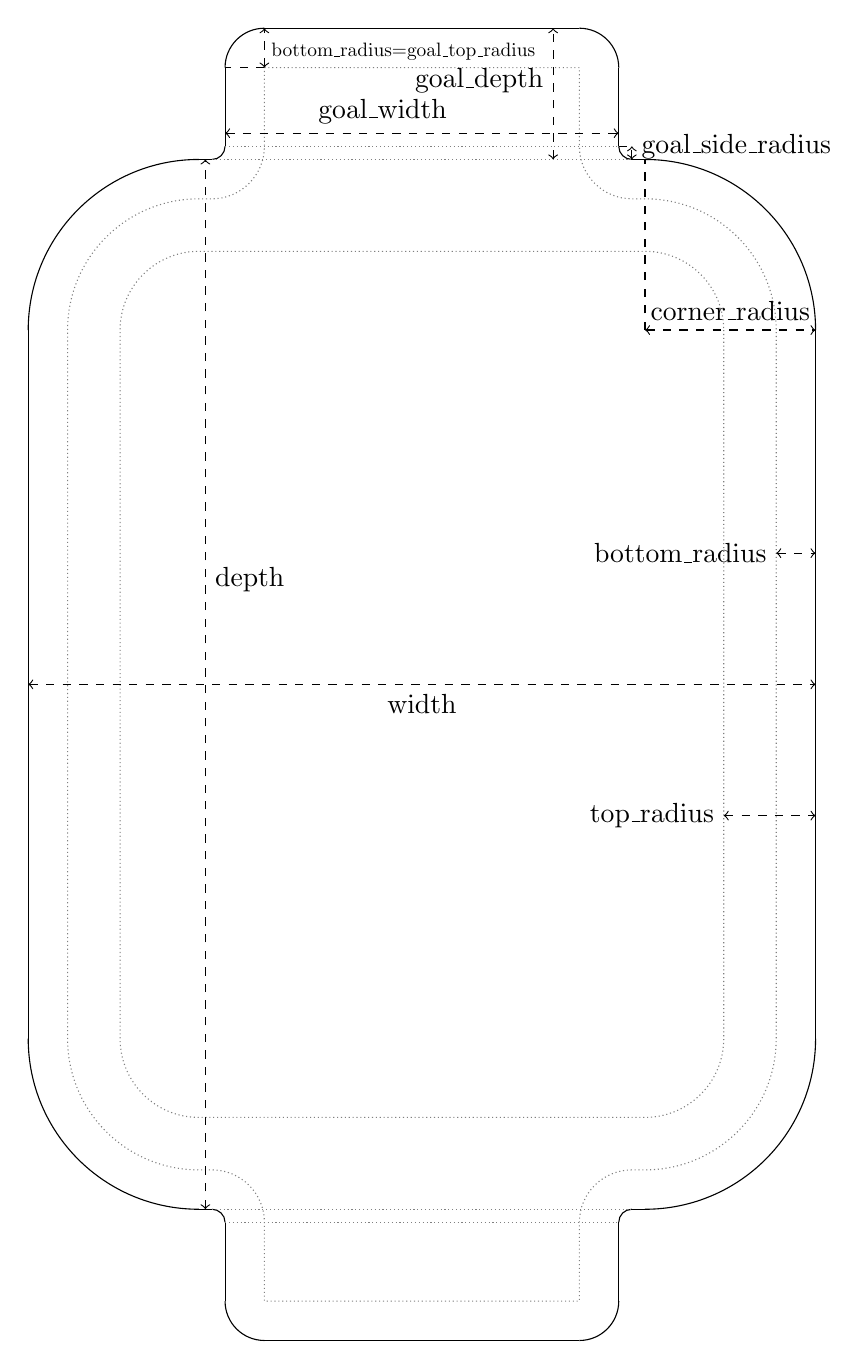
\begin{tikzpicture}[scale=1/6]
      \draw (30,40-13) arc(0:90:13);
      \draw (-30+13,40) arc(90:180:13);
      \draw (-30,-40+13) arc(180:270:13);
      \draw (30-13,-40) arc(270:360:13);
      \draw (30,40-13) -- (30,-40+13);
      \draw (-30,40-13) -- (-30,-40+13);

      \draw (30-13,40) -- (15+1,40);
      \draw (15+1,40) arc(270:180:1);
      \draw (15,41) -- (15,50-3);
      \draw (15,50-3) arc(0:90:3);
      \draw (15-3,50) -- (-15+3,50);
      \draw (-15+3,50) arc(90:180:3);
      \draw (-15,50-3) -- (-15,40+1);
      \draw (-15,40+1) arc(0:-90:1);
      \draw (-16,40) -- (-30+13,40);

      \draw (30-13,-40) -- (15+1,-40);
      \draw (15+1,-40) arc(90:180:1);
      \draw (15,-41) -- (15,-50+3);
      \draw (15,-50+3) arc(0:-90:3);
      \draw (15-3,-50) -- (-15+3,-50);
      \draw (-15+3,-50) arc(270:180:3);
      \draw (-15,-50+3) -- (-15,-40-1);
      \draw (-15,-40-1) arc(0:90:1);
      \draw (-16,-40) -- (-30+13,-40);

      \draw[gray,densely dotted,thin] (-15+3,50-3) -- (15-3,50-3)
            -- (15-3,40+1)
            arc(180:270:3+1)
            -- (30-13,40-3)
            arc(90:0:13-3)
            -- (30-3,-40+13)
            arc(0:-90:13-3)
            -- (15+1,-40+3)
            arc(90:180:3+1)
            -- (15-3,-50+3)
            -- (-15+3,-50+3)
            -- (-15+3,-40-1)
            arc(0:90:3+1)
            -- (-30+13,-40+3)
            arc(270:180:13-3)
            -- (-30+3,40-13)
            arc(180:90:13-3)
            -- (-15-1,40-3)
            arc(-90:0:3+1)
            -- (-15+3,50-3);

      \draw[gray,densely dotted,thin] (30-7,40-13)
            -- (30-7,-40+13)
            arc(0:-90:13-7)
            -- (-30+13,-40+7)
            arc(-90:-180:13-7)
            -- (-30+7,40-13)
            arc(180:90:13-7)
            -- (30-13,40-7)
            arc(90:0:13-7);
      \draw[gray,densely dotted,thin] (-15,40+1) -- (15,40+1);
      \draw[gray,densely dotted,thin] (-15,-40-1) -- (15,-40-1);
      \draw[gray,densely dotted,thin] (-15-1,-40) -- (15+1,-40);

      \draw[<->,dashed] (30-3,10) -- (30,10)
            node[pos=0,left]{bottom\_radius};
      \draw[<->,dashed] (30-7,-10) -- (30,-10)
            node[pos=0,left]{top\_radius};
      \draw[<->,dashed] (30-13,40-13) -- (30,40-13)
            node[pos=0.5,above]{corner\_radius};
      \draw[dashed,thin] (30-13,40-13) -- (30-13,40);
      \draw[<->,dashed] (-30,0) -- (30,0)
            node[pos=0.5,below]{width};
      \draw[<->,dashed] (-16.5,-40) -- (-16.5,40)
            node[pos=0.6,right]{depth};
      \draw[<->,dashed] (15+1,40) -- (15+1,40+1)
            node[pos=1,right]{goal\_side\_radius};
      \draw[dashed,thin] (15,40+1) -- (15+1,40+1);
      \draw[<->,dashed] (-15,42) -- (15,42)
            node[pos=0.4,above]{goal\_width};
      \draw[<->,dashed] (10,40) -- (10,50)
            node[pos=0.6,left]{goal\_depth};
      \draw[gray,densely dotted,thin] (-15-1,40) -- (15+1,40);
      \draw[<->,dashed] (-15+3,50-3) -- (-15+3,50)
            node[pos=0.4,right,scale=0.7]{bottom\_radius=goal\_top\_radius};
      \draw[dashed,thin] (-15+3,50-3) -- (-15,50-3);
\end{tikzpicture}
\caption{Вид сверху}
\end{figure}

\begin{figure}[H]
\centering
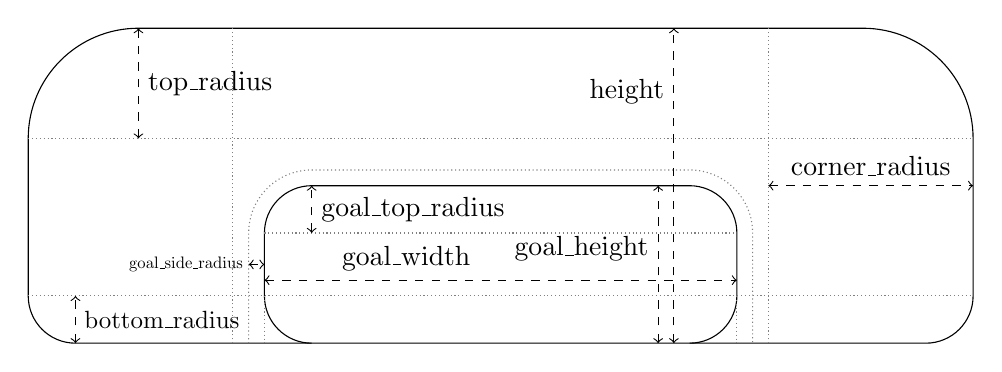
\begin{tikzpicture}[scale=1/5]
      \draw
            (-30,3)
            -- (-30,20-7)
            arc(180:90:7)
            -- (30-7,20)
            arc(90:0:7)
            -- (30,3)
            arc(0:-90:3)
            -- (-30+3,0)
            arc(-90:-180:3);
      
      \draw
            (-15+3,0)
            arc(-90:-180:3)
            -- (-15,10-3)
            arc(180:90:3)
            -- (15-3,10)
            arc(90:0:3)
            -- (15,3)
            arc(0:-90:3);

      \draw[gray,densely dotted,thin]
            (-30,20-7)--(30,20-7);
      \draw[gray,densely dotted,thin]
            (-30,3) -- (30,3);
      \draw[gray,densely dotted,thin]
            (-15,10-3) -- (15,10-3);
      \draw[gray,densely dotted,thin]
            (-15,3) -- (-15,0);
      \draw[gray,densely dotted,thin]
            (15,3) -- (15,0);
      \draw[gray,densely dotted,thin]
            (-15-1,0)
            -- (-15-1,10-3)
            arc(180:90:3+1)
            -- (15-3,10+1)
            arc(90:0:3+1)
            -- (15+1,0);
      \draw[gray,densely dotted,thin] (-30+13,0) -- (-30+13,20);
      \draw[gray,densely dotted,thin] (30-13,0) -- (30-13,20);

      \draw[<->,dashed] (30-13,10) -- (30,10)
            node[pos=0.5,above]{corner\_radius};
      \draw[<->,dashed] (-30+7,20-7) -- (-30+7,20)
            node[pos=0.5,right]{top\_radius};
      \draw[<->,dashed] (-30+3,0) -- (-30+3,3)
            node[pos=0.5,right,scale=0.9]{bottom\_radius};
      \draw[<->,dashed] (-15-1,5) -- (-15,5)
            node[pos=0.0,left,scale=0.6]{goal\_side\_radius};
      \draw[<->,dashed] (-15,4) -- (15,4)
            node[pos=0.3,above]{goal\_width};
      \draw[<->,dashed] (10,0) -- (10,10)
            node[pos=0.6,left]{goal\_height};
      \draw[<->,dashed] (-15+3,10-3) -- (-15+3,10)
            node[pos=0.5,right]{goal\_top\_radius};
      \draw[<->,dashed] (11,0) -- (11,20)
            node[pos=0.8,left]{height};
\end{tikzpicture}
\caption{Вид на ворота}
\end{figure}

\section{Мяч и роботы}

Мяч является шаром с радиусом \const{BALL\_RADIUS} и массой \const{BALL\_MASS}.
Коэффициент восстановления\footnote{
      Коэффициент восстановления --- коэффициент,
      задающий долю относительной скорости объектов при столкновении,
      которая восстанавливается после удара
} при столкновении мяча с ареной равен \const{BALL\_ARENA\_E},
таким образом мяч теряет часть своей скорости при столкновении.

В начале симуляции мяч находится в центре арены на случайной высоте в отрезке
$[\const{BALL\_RADIUS} .. 4\times\const{BALL\_RADIUS}]$.

Мяч считается забитым, если полностью находится за линией ворот:
\begin{equation}
      abs(ball.z)>arena.depth/2+ball.radius
\end{equation}
После забитого гола симуляция начинается заново через \const{RESET\_TICKS} тиков.

Роботы также являются шарами (массой \const{ROBOT\_MASS}), но их радиус может меняться от
\const{ROBOT\_MIN\_RADIUS} до \const{ROBOT\_MAX\_RADIUS},
и изменяется при использовании прыжка.
Чем выше установлена скорость прыжка робота, тем больше его радиус.
Точная формула:
\begin{equation}
	\begin{split}
		&radius=\const{ROBOT\_MIN\_RADIUS}+\\
		&(\const{ROBOT\_MAX\_RADIUS}-\const{ROBOT\_MIN\_RADIUS})\times\frac{jump\_speed}{\const{ROBOT\_MAX\_JUMP\_SPEED}}
	\end{split}
\end{equation}

Небольшое увеличение радиуса при прыжке дает роботам возможность отпрыгивать от стен арены.

Также, при прыжке, физический симулятор считает, что радиус робота изменяется с заданной скоростью прыжка
(несмотря на то, что радиус на самом деле вычисляется по формуле, представленной выше).
За счет этого и происходит сам прыжок.
Таким образом, помимо возможности подпрыгивать, скорость прыжка также влияет на силу удара по мячу.

Коэффициент восстановления при столкновении робота с ареной равен $0$,
то есть этот вид столкновения является абсолютно неупругим.
При столкновении робота с мячом, или с другим роботом,
коэффициент восстановления выбирается равновероятно от \const{MIN\_HIT\_E} до \const{MAX\_HIT\_E}.

\section{Нитро}

Начиная со второго раунда, роботам будет доступно нитро.
Нитро позволяет придать ускорения роботу, в любом направлении.
Максимальный запас нитро равен \const{MAX\_NITRO\_AMOUNT}, одна единица нитро меняет скорость на \const{NITRO\_POINT\_VELOCITY\_CHANGE}.
Ускорение при использовании нитро не может превышать \const{ROBOT\_NITRO\_ACCELERATION}.

Пополнять запас нитро можно подбирая рюкзаки с нитро.
Рюкзаки являются шарами радиуса \const{NITRO\_PACK\_RADIUS} и считаются подобранными,
если расстояние между центром робота и центром рюкзака меньше суммы их радиусов.
Каждый рюкзак с нитро восстанавливает запас полностью (до $100$).
После подбирания, рюкзак снова появится в том же месте через \const{NITRO\_RESPAWN\_TICKS} тиков.
Всего на арене появляется $4$ рюкзака с нитро, в точках с координатами $(\pm\ x, 1, \pm z)$.

В начале игры и после каждого гола запас нитро всех роботов равен \const{START\_NITRO\_AMOUNT}.

В первом раунде запас нитро всегда равен $0$, и рюкзаки с нитро на арене не появляются.

\section{Управление}

Управление роботом состоит в задании желаемого вектора скорости, скорости прыжка, и желании использовать нитро.

Не считая нитро, если робот соприкасается с ареной, то
его скорость будет стремится к желаемой скорости, спроецированной на плоскость соприкосновения.
Ускорение не может превышать \const{ROBOT\_ACCELERATION}.
При этом, чем более вертикальная поверхность, тем меньше ускорение в желаемую сторону
(также, если робот касается арены своей верхней половиной, ускорение равно нулю).
То есть, при соприкосновении с полом, ускорение максимальное, а при соприкосновении со стеной или потолком, нулевое.

При использовании нитро, скорость также стремится к желаемой, однако уже независимо от соприкосновения с ареной.

Скорость прыжка можно задать любую от $0$ (не прыгать) до \const{ROBOT\_MAX\_JUMP\_SPEED} (прыжок с максимальной скоростью).
При прыжке радиус робота немного увеличивается, позволяя ему отпрыгивать от стен.
Также при прыжке физический симулятор считает, что радиус робота изменяется со скоростью, равной заданной скорости прыжка.
То есть, прыжок осуществляется за счет того, что при столкновении с полом
относительная скорость в точке соприкосновения равна скорости прыжка.
Таким образом, также можно контролировать силу удара по мячу.
